This chapter consists of two parts. The first part will provide an evaluation of the Matrix security model and relies heavily on the paper \emph{A Formal Security Analysis of the Signal Messaging Protocol} \cite{Signal} and \emph{The Olm Cryptographic Review} by NCC Group \cite{ncc}. The second part provides a preliminary analysis of the IFC tools, the selection of Paragon and the rationale behind it, and a further analysis of the selected tool Paragon.


\section{Evaluation of Matrix security model}

Matrix provides end-to-end encryption by using the Olm and Megolm library with the former being an implementation of the Double Ratchet algorithm known from Signal Protocol, and the latter being the algorithm used for group chat. 
%As mentioned in xx Matrix uses the Megolm library for group chat. which is layered on top of the Olm library.

The evaluation will focus on the cryptographic protocols used by Matrix. By evaluating Signal's cryptographic protocol we can derive the same evaluation for the Olm library. The evaluation is extended by examining the the cryptographic review of Olm and Megolm by NCC Group. 

\subsection{Overview of the Double Ratchet algorithm}

Before the Double Ratchet algorithm can 

\subsubsection{Triple Deffie-Hellman}

\begin{figure}[H]
	\centering
	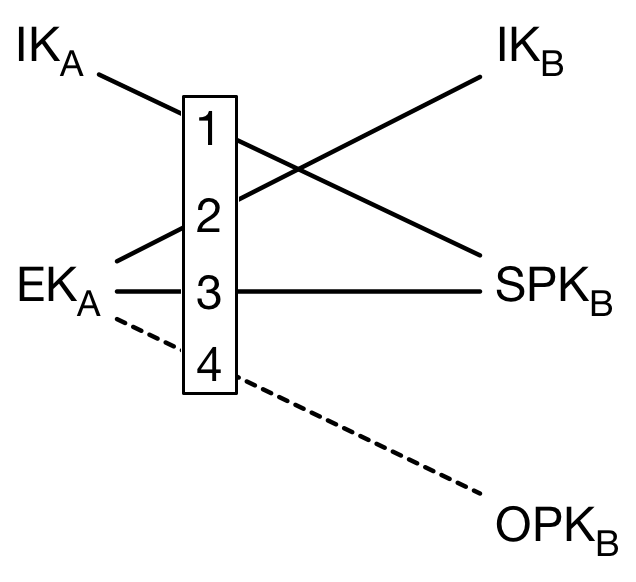
\includegraphics{figures/tripledh.png}
	\caption{Diffie-Hellman between keys \cite{tripledh}.}
	\label{fig:tripledh}
\end{figure}

\subsubsection{KDF chain}

\begin{figure}[H]
	\centering
	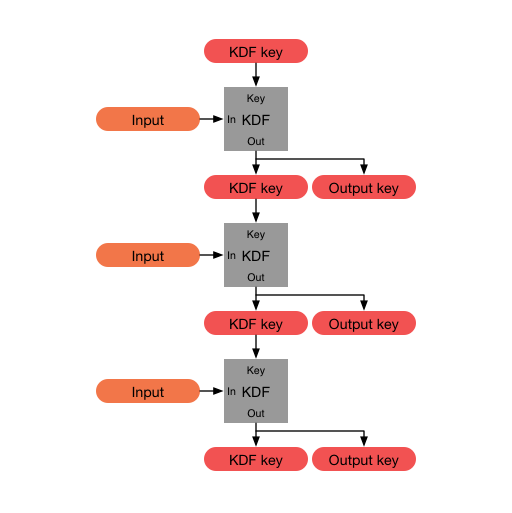
\includegraphics[width=10cm]{figures/kdfchain.png}
	\caption{Processing of three inputs and the resulting outputs in KDF chain \cite{doubleratchet}.}
	\label{fig:kdfchain}
\end{figure}

\subsubsection{Symmetric ratchet}

\begin{figure}[H]
	\centering
	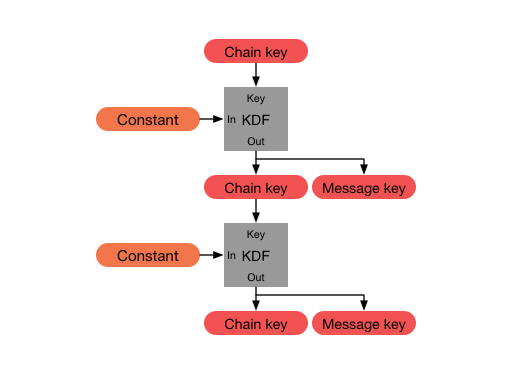
\includegraphics[width=10cm]{figures/symmetrickeyratchet.png}
	\caption{Symmetric key ratchet \cite{doubleratchet}.}
	\label{fig:symkeyratchet}
\end{figure}

\subsubsection{Deffie-Hellman ratchet}

\begin{figure}[H]
	\centering
	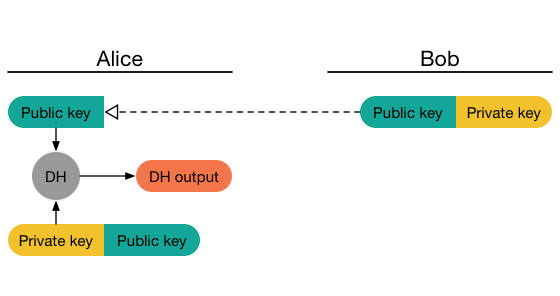
\includegraphics[width=10cm]{figures/dhratchet1.png}
	\caption{Diffie-Hellman ratchet 1 \cite{doubleratchet}.}
	\label{fig:dhratchet1}
\end{figure}

\begin{figure}[H]
	\centering
	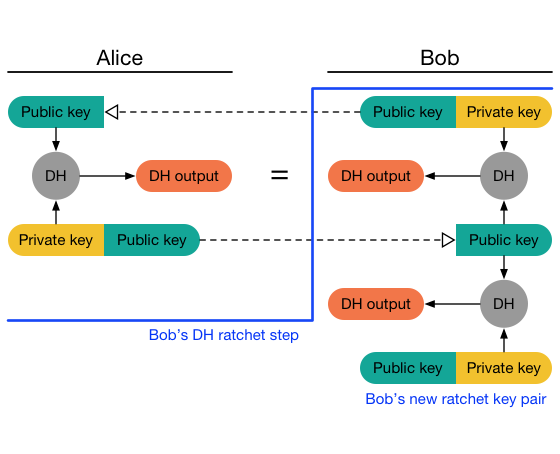
\includegraphics[width=10cm]{figures/dhratchet2.png}
	\caption{Diffie-Hellman ratchet 2 \cite{doubleratchet}.}
	\label{fig:dhratchet2}
\end{figure}

\begin{figure}[H]
	\centering
	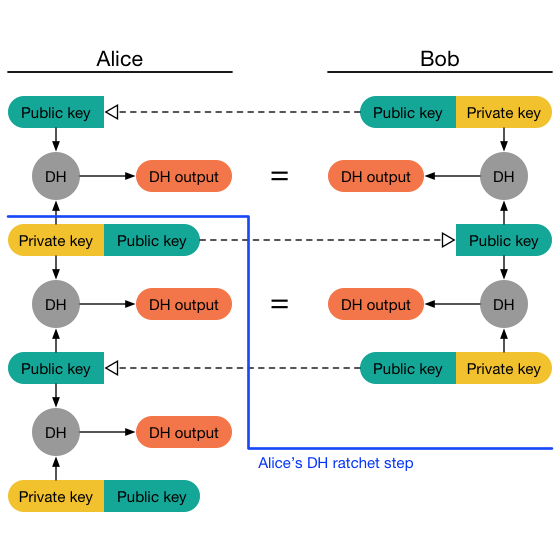
\includegraphics[width=10cm]{figures/dhratchet3.png}
	\caption{Diffie-Hellman ratchet 3 \cite{doubleratchet}.}
	\label{fig:dhratchet3}
\end{figure}

\begin{figure}[H]
	\centering
	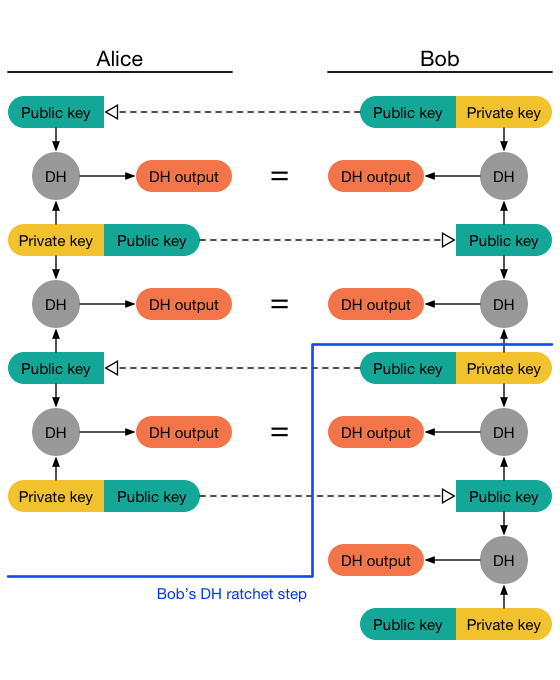
\includegraphics[width=10cm]{figures/dhratchet4.png}
	\caption{Diffie-Hellman ratchet 4 \cite{doubleratchet}.}
	\label{fig:dhratchet4}
\end{figure}

\begin{figure}[H]
	\centering
	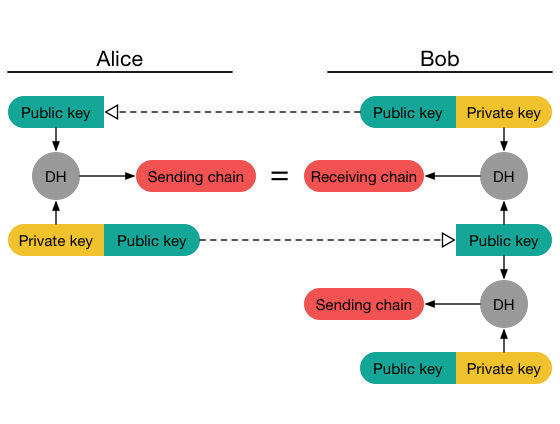
\includegraphics[width=10cm]{figures/dhratchet5.png}
	\caption{Diffie-Hellman ratchet 5 \cite{doubleratchet}.}
	\label{fig:dhratchet5}
\end{figure}

\begin{figure}[H]
	\centering
	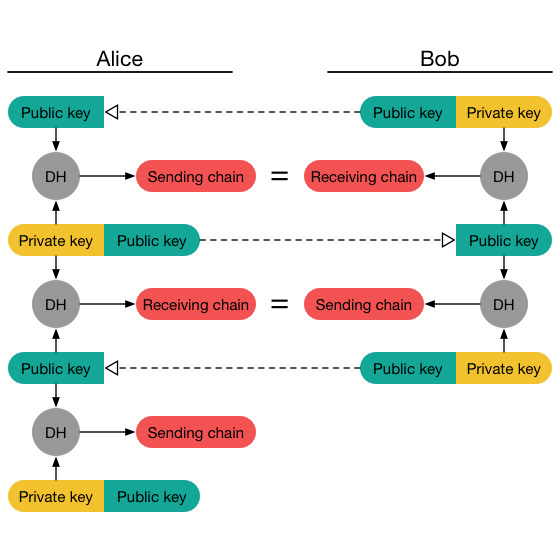
\includegraphics[width=10cm]{figures/dhratchet6.png}
	\caption{Diffie-Hellman ratchet 6 \cite{doubleratchet}.}
	\label{fig:dhratchet6}
\end{figure}

\begin{figure}[H]
	\centering
	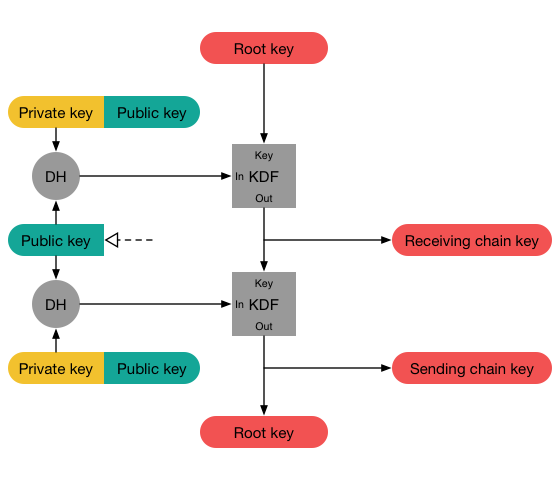
\includegraphics[width=10cm]{figures/dhratchet7.png}
	\caption{Diffie-Hellman ratchet 7 \cite{doubleratchet}.}
	\label{fig:dhratchet7}
\end{figure}

\subsubsection{Double ratchet}
\begin{figure}[H]
	\centering
	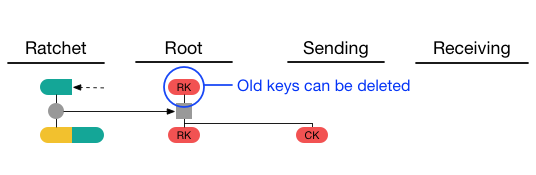
\includegraphics[width=10cm]{figures/doubleratchet1.png}
	\caption{Double ratchet 1 \cite{doubleratchet}.}
	\label{fig:doubleratchet1}
\end{figure}

\begin{figure}[H]
	\centering
	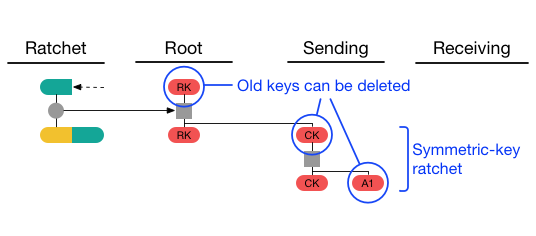
\includegraphics[width=10cm]{figures/doubleratchet2.png}
	\caption{Double ratchet 2 \cite{doubleratchet}.}
	\label{fig:doubleratchet2}
\end{figure}

\begin{figure}[H]
	\centering
	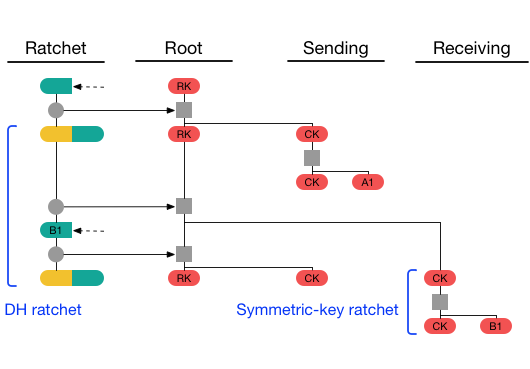
\includegraphics[width=10cm]{figures/doubleratchet3.png}
	\caption{Double ratchet 3 \cite{doubleratchet}.}
	\label{fig:doubleratchet3}
\end{figure}

\begin{figure}[H]
	\centering
	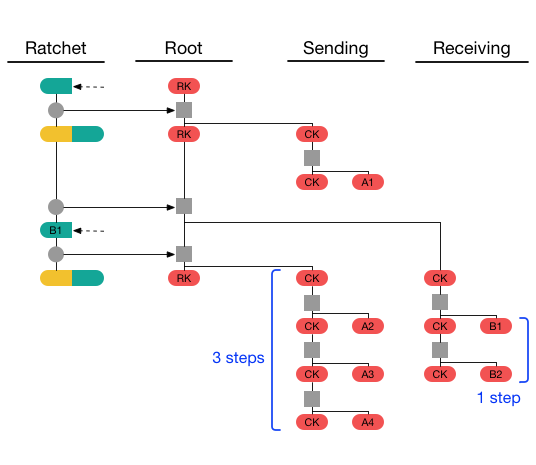
\includegraphics[width=10cm]{figures/doubleratchet4.png}
	\caption{Double ratchet 4 \cite{doubleratchet}.}
	\label{fig:doubleratchet4}
\end{figure}

\begin{figure}[H]
	\centering
	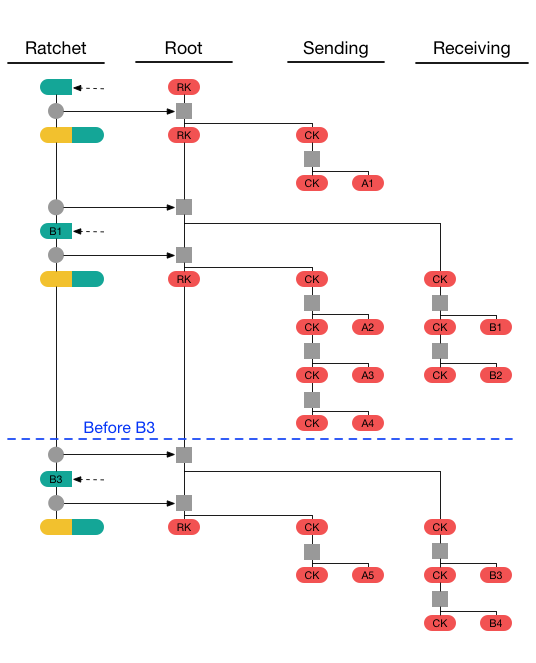
\includegraphics[width=10cm]{figures/doubleratchet5.png}
	\caption{Double ratchet 5 \cite{doubleratchet}.}
	\label{fig:doubleratchet5}
\end{figure}

\subsection{Security model and analysis}

\subsubsection{Threat model}

\subsubsection{Multi-State Key Exchange Protocol}

\subsubsection{Key Indistinguishability Experiment}

\subsubsection{Freshness}

\paragraph{Stage 0}

\paragraph{Asymmetric stages}

\paragraph{Symmetric stages}

\subsubsection{Proof}

% Definitions of hardness assumptions. Should I include it?

\subsubsection{Application variants}

The Olm library used by Matrix is a variant of the Double Ratchet algorithm. The custom variants invites important changes in need to be analyzed independently. WhatsApp variant of the protocol has a retransmission mechanism which is vulnerable. 
% if Bob appears to change his identity key, clients will resend messages encrypted under the new value.Hence, an adversary with control over identity registration can disconnect Bob and replace his key, and Alice will re-send the message to the adversary.  
The further evaluation relies upon the the security assessment on Matrix. 

\subsection{Matrix protocol}

The Double Ratchet algorithm is meant for one-to-one chatting and is not practical for group chatting? %why not?
For direct conversation Matrix uses Olm library which is an implementation of the Double Ratchet algorithm. For group chats the Megolm library is used. With Group chats 
Instead for group chats the Mego

The rooms in Matrix are meant for group chats. 

\subsubsection{Olm}
Vulnerabilities found in the security assessment. 

\paragraph{Unknown Key Share attack}

\subsubsection{Megolm}
% Lack of backward secrecy is problematic for the prototype.

%Enforcing new session start every time a patient journal is sent. Could it be enforced with IFC?
 
\subsubsection{End-to-end security}
Having established that Matrix security model is sufficient.

\subsection{Summary}



% Tools issue: java sdk for matrix is beta and not fully implemented. 
% Best supported sdk is for javascript or python. Problem of running javascript code or python code with Paragon (java)
% Maybe better to use JSFlow instead 


\section{Survey of IFC Tools}

\subsection{JIF}

\subsection{Paragon}

\subsection{JSFlow}
Not possible to use Matrix library with JSFlow because of missing support for libaries such as require (in node). Also overhead with configuring JSFlow to be the interpretor.

Swift, SIF, FlowR, JFlow, LIO


\subsection{Selection of IFC tool}
The selection of the IFC tool used for developing the prototype is based the following defined parameters.
The selection of IFC tool put emphasis on the practical usage in combination with Matrix. 

\subsection{Paragon analysis}

\subsection{Summary}


\section{Summary}
In this chapter the Matrix security model has been evaluated. Matrix provides end-to-end security and uses the Double Ratchet algorithm by Signal. The evaluation found that there are no major flaws in the design. To achieve end-to-end security the endpoints need to be secured as well \cite{Sabelfeld2003} this leads us to the chapter's second part. The chapter analyzed information-flow control tools and justifies the selection of Paragon which the prototype is programmed in. 